\documentclass[12pt,reqno]{amsart}
%\documentclass[../Solutions_Introduction_to_Algorithms.tex]{subfiles}
\usepackage{amsmath,amsfonts,amscd,amssymb,epsf,color,enumerate,graphicx,url}
\usepackage{algorithm, algorithmic}
\usepackage{forest, tikz, xcolor}
\usetikzlibrary{matrix, positioning}
\setlength{\oddsidemargin}{-0.2in}%
\setlength{\evensidemargin}{-0.2in}%
\setlength{\textwidth}{6.6in}%
\setlength{\topmargin}{-0.5in}%
 \setlength{\textheight}{9.5in}%
 \definecolor{orange}{rgb}{1,0.5,0}
 \pagestyle{plain}
\linespread{1.3}
\usepackage[small]{caption}
\newcommand{\pa}{\partial}
\newcommand{\va}{\vspace{0.4cm}}
\newcommand{\di}{\displaystyle}
\newcommand{\disp}{\displaystyle}


% turn on \answertrue to show the solution
% turn on \answerfalse to hide the solution
\newif\ifanswer
\answertrue
%\answerfalse



\begin{document}
\noindent {\footnotesize Introduction to Algorithms}\hspace{10.5cm} {\footnotesize Solutions}

\vspace{0.5cm}
\hspace{5.5cm}\textbf{\large Exercises in Section 7.1}
\vspace{0.5cm}

\begin{enumerate}[1.]

\item Using Figure 7.1 as a model, illustrate the operation of $\textsc{Partition}$ on the array $A = \langle 13, 19, 9, 5, 12, 8, 7, 4, 21, 2, 6, 11 \rangle$.

\ifanswer
\noindent {\bf Solution}
\begin{center}
\begin{tikzpicture}
    \matrix[matrix of nodes,
            nodes={draw, minimum width=0.7cm, minimum height=0.7cm, anchor=center},
            column sep=0pt, row sep=0pt,
            name=m1] 
    {
        \node[fill=none, draw=none, name=m1-0] {~}; &
        \node[fill=lightgray, name=m1-1] {13}; &
        \node[fill=lightgray, name=m1-2] {19}; &
        \node[fill=lightgray, name=m1-3] {9}; &
        \node[fill=lightgray, name=m1-4] {5}; &
        \node[fill=lightgray, name=m1-5] {12}; &
        \node[fill=lightgray, name=m1-6] {8}; &
        \node[fill=lightgray, name=m1-7] {7}; &
        \node[fill=lightgray, name=m1-8] {4}; &
        \node[fill=lightgray, name=m1-9] {21}; &
        \node[fill=lightgray, name=m1-10] {2}; &
        \node[fill=lightgray, name=m1-11] {6}; &
        \node[fill=yellow, name=m1-12] {11}; \\
    };
    \node[above=2pt of m1-0] {\textit{i}};
    \node[above=2pt of m1-1] {\textit{p,j}};
    \node[above=2pt of m1-12] {\textit{r}};


    \matrix[matrix of nodes,
            nodes={draw, minimum width=0.7cm, minimum height=0.7cm, anchor=center},
            column sep=0pt, row sep=0pt,
            below=0.5cm of m1,
            name=m2] 
    {
        \node[fill=none, draw=none, name=m2-0] {~}; &
        \node[fill=cyan, name=m2-1] {13}; &
        \node[fill=lightgray, name=m2-2] {19}; &
        \node[fill=lightgray, name=m2-3] {9}; &
        \node[fill=lightgray, name=m2-4] {5}; &
        \node[fill=lightgray, name=m2-5] {12}; &
        \node[fill=lightgray, name=m2-6] {8}; &
        \node[fill=lightgray, name=m2-7] {7}; &
        \node[fill=lightgray, name=m2-8] {4}; &
        \node[fill=lightgray, name=m2-9] {21}; &
        \node[fill=lightgray, name=m2-10] {2}; &
        \node[fill=lightgray, name=m2-11] {6}; &
        \node[fill=yellow, name=m2-12] {11}; \\
    };
    \node[above=2pt of m2-0] {\textit{i}};
    \node[above=2pt of m2-1] {\textit{p}};
    \node[above=2pt of m2-2] {\textit{j}};
    \node[above=2pt of m2-12] {\textit{r}};


    \matrix[matrix of nodes,
            nodes={draw, minimum width=0.7cm, minimum height=0.7cm, anchor=center},
            column sep=0pt, row sep=0pt,
            below=0.5cm of m2,
            name=m3] 
    {
        \node[fill=none, draw=none, name=m3-0] {~}; &
        \node[fill=cyan, name=m3-1] {13}; &
        \node[fill=cyan, name=m3-2] {19}; &
        \node[fill=lightgray, name=m3-3] {9}; &
        \node[fill=lightgray, name=m3-4] {5}; &
        \node[fill=lightgray, name=m3-5] {12}; &
        \node[fill=lightgray, name=m3-6] {8}; &
        \node[fill=lightgray, name=m3-7] {7}; &
        \node[fill=lightgray, name=m3-8] {4}; &
        \node[fill=lightgray, name=m3-9] {21}; &
        \node[fill=lightgray, name=m3-10] {2}; &
        \node[fill=lightgray, name=m3-11] {6}; &
        \node[fill=yellow, name=m3-12] {11}; \\
    };
    \node[above=2pt of m3-0] {\textit{i}};
    \node[above=2pt of m3-1] {\textit{p}};
    \node[above=2pt of m3-3] {\textit{j}};
    \node[above=2pt of m3-12] {\textit{r}};


    \matrix[matrix of nodes,
            nodes={draw, minimum width=0.7cm, minimum height=0.7cm, anchor=center},
            column sep=0pt, row sep=0pt,
            below=0.5cm of m3,
            name=m4] 
    {
        \node[fill=none, draw=none, name=m4-0] {~}; &
        \node[fill=pink, name=m4-1] {9}; &
        \node[fill=cyan, name=m4-2] {19}; &
        \node[fill=cyan, name=m4-3] {13}; &
        \node[fill=lightgray, name=m4-4] {5}; &
        \node[fill=lightgray, name=m4-5] {12}; &
        \node[fill=lightgray, name=m4-6] {8}; &
        \node[fill=lightgray, name=m4-7] {7}; &
        \node[fill=lightgray, name=m4-8] {4}; &
        \node[fill=lightgray, name=m4-9] {21}; &
        \node[fill=lightgray, name=m4-10] {2}; &
        \node[fill=lightgray, name=m4-11] {6}; &
        \node[fill=yellow, name=m4-12] {11}; \\
    };
    \node[above=2pt of m4-1] {\textit{p,i}};
    \node[above=2pt of m4-4] {\textit{j}};
    \node[above=2pt of m4-12] {\textit{r}};


    \matrix[matrix of nodes,
            nodes={draw, minimum width=0.7cm, minimum height=0.7cm, anchor=center},
            column sep=0pt, row sep=0pt,
            below=0.5cm of m4,
            name=m5] 
    {
        \node[fill=none, draw=none, name=m5-0] {~}; &
        \node[fill=pink, name=m5-1] {9}; &
        \node[fill=pink, name=m5-2] {5}; &
        \node[fill=cyan, name=m5-3] {13}; &
        \node[fill=cyan, name=m5-4] {19}; &
        \node[fill=lightgray, name=m5-5] {12}; &
        \node[fill=lightgray, name=m5-6] {8}; &
        \node[fill=lightgray, name=m5-7] {7}; &
        \node[fill=lightgray, name=m5-8] {4}; &
        \node[fill=lightgray, name=m5-9] {21}; &
        \node[fill=lightgray, name=m5-10] {2}; &
        \node[fill=lightgray, name=m5-11] {6}; &
        \node[fill=yellow, name=m5-12] {11}; \\
    };
    \node[above=2pt of m5-1] {\textit{p}};
    \node[above=2pt of m5-2] {\textit{i}};
    \node[above=2pt of m5-5] {\textit{j}};
    \node[above=2pt of m5-12] {\textit{r}};


    \matrix[matrix of nodes,
            nodes={draw, minimum width=0.7cm, minimum height=0.7cm, anchor=center},
            column sep=0pt, row sep=0pt,
            below=0.5cm of m5,
            name=m6] 
    {
        \node[fill=none, draw=none, name=m6-0] {~}; &
        \node[fill=pink, name=m6-1] {9}; &
        \node[fill=pink, name=m6-2] {5}; &
        \node[fill=cyan, name=m6-3] {13}; &
        \node[fill=cyan, name=m6-4] {19}; &
        \node[fill=cyan, name=m6-5] {12}; &
        \node[fill=lightgray, name=m6-6] {8}; &
        \node[fill=lightgray, name=m6-7] {7}; &
        \node[fill=lightgray, name=m6-8] {4}; &
        \node[fill=lightgray, name=m6-9] {21}; &
        \node[fill=lightgray, name=m6-10] {2}; &
        \node[fill=lightgray, name=m6-11] {6}; &
        \node[fill=yellow, name=m6-12] {11}; \\
    };
    \node[above=2pt of m6-1] {\textit{p}};
    \node[above=2pt of m6-2] {\textit{i}};
    \node[above=2pt of m6-6] {\textit{j}};
    \node[above=2pt of m6-12] {\textit{r}};


    \matrix[matrix of nodes,
            nodes={draw, minimum width=0.7cm, minimum height=0.7cm, anchor=center},
            column sep=0pt, row sep=0pt,
            below=0.5cm of m6,
            name=m7] 
    {
        \node[fill=none, draw=none, name=m7-0] {~}; &
        \node[fill=pink, name=m7-1] {9}; &
        \node[fill=pink, name=m7-2] {5}; &
        \node[fill=pink, name=m7-3] {8}; &
        \node[fill=cyan, name=m7-4] {19}; &
        \node[fill=cyan, name=m7-5] {12}; &
        \node[fill=cyan, name=m7-6] {13}; &
        \node[fill=lightgray, name=m7-7] {7}; &
        \node[fill=lightgray, name=m7-8] {4}; &
        \node[fill=lightgray, name=m7-9] {21}; &
        \node[fill=lightgray, name=m7-10] {2}; &
        \node[fill=lightgray, name=m7-11] {6}; &
        \node[fill=yellow, name=m7-12] {11}; \\
    };
    \node[above=2pt of m7-1] {\textit{p}};
    \node[above=2pt of m7-3] {\textit{i}};
    \node[above=2pt of m7-7] {\textit{j}};
    \node[above=2pt of m7-12] {\textit{r}};


    \matrix[matrix of nodes,
            nodes={draw, minimum width=0.7cm, minimum height=0.7cm, anchor=center},
            column sep=0pt, row sep=0pt,
            below=0.5cm of m7,
            name=m8] 
    {
        \node[fill=none, draw=none, name=m8-0] {~}; &
        \node[fill=pink, name=m8-1] {9}; &
        \node[fill=pink, name=m8-2] {5}; &
        \node[fill=pink, name=m8-3] {8}; &
        \node[fill=pink, name=m8-4] {7}; &
        \node[fill=cyan, name=m8-5] {12}; &
        \node[fill=cyan, name=m8-6] {13}; &
        \node[fill=cyan, name=m8-7] {19}; &
        \node[fill=lightgray, name=m8-8] {4}; &
        \node[fill=lightgray, name=m8-9] {21}; &
        \node[fill=lightgray, name=m8-10] {2}; &
        \node[fill=lightgray, name=m8-11] {6}; &
        \node[fill=yellow, name=m8-12] {11}; \\
    };
    \node[above=2pt of m8-1] {\textit{p}};
    \node[above=2pt of m8-4] {\textit{i}};
    \node[above=2pt of m8-8] {\textit{j}};
    \node[above=2pt of m8-12] {\textit{r}};


    \matrix[matrix of nodes,
            nodes={draw, minimum width=0.7cm, minimum height=0.7cm, anchor=center},
            column sep=0pt, row sep=0pt,
            below=0.5cm of m8,
            name=m9] 
    {
        \node[fill=none, draw=none, name=m9-0] {~}; &
        \node[fill=pink, name=m9-1] {9}; &
        \node[fill=pink, name=m9-2] {5}; &
        \node[fill=pink, name=m9-3] {8}; &
        \node[fill=pink, name=m9-4] {7}; &
        \node[fill=pink, name=m9-5] {4}; &
        \node[fill=cyan, name=m9-6] {13}; &
        \node[fill=cyan, name=m9-7] {19}; &
        \node[fill=cyan, name=m9-8] {12}; &
        \node[fill=lightgray, name=m9-9] {21}; &
        \node[fill=lightgray, name=m9-10] {2}; &
        \node[fill=lightgray, name=m9-11] {6}; &
        \node[fill=yellow, name=m9-12] {11}; \\
    };
    \node[above=2pt of m9-1] {\textit{p}};
    \node[above=2pt of m9-5] {\textit{i}};
    \node[above=2pt of m9-9] {\textit{j}};
    \node[above=2pt of m9-12] {\textit{r}};


    \matrix[matrix of nodes,
            nodes={draw, minimum width=0.7cm, minimum height=0.7cm, anchor=center},
            column sep=0pt, row sep=0pt,
            below=0.5cm of m9,
            name=m10] 
    {
        \node[fill=none, draw=none, name=m10-0] {~}; &
        \node[fill=pink, name=m10-1] {9}; &
        \node[fill=pink, name=m10-2] {5}; &
        \node[fill=pink, name=m10-3] {8}; &
        \node[fill=pink, name=m10-4] {7}; &
        \node[fill=pink, name=m10-5] {4}; &
        \node[fill=cyan, name=m10-6] {13}; &
        \node[fill=cyan, name=m10-7] {19}; &
        \node[fill=cyan, name=m10-8] {12}; &
        \node[fill=cyan, name=m10-9] {21}; &
        \node[fill=lightgray, name=m10-10] {2}; &
        \node[fill=lightgray, name=m10-11] {6}; &
        \node[fill=yellow, name=m10-12] {11}; \\
    };
    \node[above=2pt of m10-1] {\textit{p}};
    \node[above=2pt of m10-5] {\textit{i}};
    \node[above=2pt of m10-10] {\textit{j}};
    \node[above=2pt of m10-12] {\textit{r}};


    \matrix[matrix of nodes,
            nodes={draw, minimum width=0.7cm, minimum height=0.7cm, anchor=center},
            column sep=0pt, row sep=0pt,
            below=0.5cm of m10,
            name=m11] 
    {
        \node[fill=none, draw=none, name=m11-0] {~}; &
        \node[fill=pink, name=m11-1] {9}; &
        \node[fill=pink, name=m11-2] {5}; &
        \node[fill=pink, name=m11-3] {8}; &
        \node[fill=pink, name=m11-4] {7}; &
        \node[fill=pink, name=m11-5] {4}; &
        \node[fill=pink, name=m11-6] {2}; &
        \node[fill=cyan, name=m11-7] {19}; &
        \node[fill=cyan, name=m11-8] {12}; &
        \node[fill=cyan, name=m11-9] {21}; &
        \node[fill=cyan, name=m11-10] {13}; &
        \node[fill=lightgray, name=m11-11] {6}; &
        \node[fill=yellow, name=m11-12] {11}; \\
    };
    \node[above=2pt of m11-1] {\textit{p}};
    \node[above=2pt of m11-6] {\textit{i}};
    \node[above=2pt of m11-11] {\textit{j}};
    \node[above=2pt of m11-12] {\textit{r}};


    \matrix[matrix of nodes,
            nodes={draw, minimum width=0.7cm, minimum height=0.7cm, anchor=center},
            column sep=0pt, row sep=0pt,
            below=0.5cm of m11,
            name=m12] 
    {
        \node[fill=none, draw=none, name=m12-0] {~}; &
        \node[fill=pink, name=m12-1] {9}; &
        \node[fill=pink, name=m12-2] {5}; &
        \node[fill=pink, name=m12-3] {8}; &
        \node[fill=pink, name=m12-4] {7}; &
        \node[fill=pink, name=m12-5] {4}; &
        \node[fill=pink, name=m12-6] {2}; &
        \node[fill=pink, name=m12-7] {6}; &
        \node[fill=cyan, name=m12-8] {12}; &
        \node[fill=cyan, name=m12-9] {21}; &
        \node[fill=cyan, name=m12-10] {13}; &
        \node[fill=cyan, name=m12-11] {19}; &
        \node[fill=yellow, name=m12-12] {11}; \\
    };
    \node[above=2pt of m12-1] {\textit{p}};
    \node[above=2pt of m12-7] {\textit{i}};
    \node[above=2pt of m12-12] {\textit{r}};


    \matrix[matrix of nodes,
            nodes={draw, minimum width=0.7cm, minimum height=0.7cm, anchor=center},
            column sep=0pt, row sep=0pt,
            below=0.5cm of m12,
            name=m13] 
    {
        \node[fill=none, draw=none, name=m13-0] {~}; &
        \node[fill=pink, name=m13-1] {9}; &
        \node[fill=pink, name=m13-2] {5}; &
        \node[fill=pink, name=m13-3] {8}; &
        \node[fill=pink, name=m13-4] {7}; &
        \node[fill=pink, name=m13-5] {4}; &
        \node[fill=pink, name=m13-6] {2}; &
        \node[fill=pink, name=m13-7] {6}; &
        \node[fill=yellow, name=m13-8] {11}; &
        \node[fill=cyan, name=m13-9] {21}; &
        \node[fill=cyan, name=m13-10] {13}; &
        \node[fill=cyan, name=m13-11] {19}; &
        \node[fill=cyan, name=m13-12] {12}; \\
    };
    \node[above=2pt of m13-1] {\textit{p}};
    \node[above=2pt of m13-7] {\textit{i}};
    \node[above=2pt of m13-12] {\textit{r}};
\end{tikzpicture}
\end{center}
\vspace{1cm}



\item What value of $q$ does $\textsc{Partition}$ return when all elements in the subarray $A[p:r]$ have the same value? Modify $\textsc{Partition}$ so that $q=\lfloor(p+r)/2\rfloor$ when all elements in the subarray $A[p:r]$ have the same value.

\ifanswer
\noindent {\bf Solution}
If all elements in the subarray $A[p:r]$ have the same value, the condition of the \textbf{if} statement will be always true. Therefore, $i$ increases by $r - p$ as there are $r - p$ iterations in total. Hence, after the \textbf{for} loop, $i = (p - 1) + (r - p) = r - 1$, and the returned value is $q = i + 1 = r$. Below is an amended program that returns $\lfloor(p+r)/2\rfloor$ when all elements in the subarray $A[p:r]$ have the same value:
\begin{algorithm}
    \caption{$\textsc{Partition'}(A, p, r)$}
    \begin{algorithmic}[1]
        \STATE $x = A[r]$
        \STATE $i = p - 1$
        \FOR{$j = p$ to $r - 1$}
            \IF{$A[j] \neq A[j + 1]$}
                \STATE \textbf{break}
            \ENDIF
            \RETURN $\lfloor(p+r)/2\rfloor$
        \ENDFOR
        \FOR{$j = p$ to $r - 1$}
            \IF{$A[j] \leq x$}
                \STATE $i = i + 1$
                \STATE exchange $A[i]$ with $A[j]$
            \ENDIF
        \ENDFOR
        \STATE exchange $A[i + 1]$ with $A[r]$
        \RETURN $i + 1$
    \end{algorithmic}
\end{algorithm}
\vspace{1cm}



\item Give a brief argument that the running time of $\textsc{Partition}$ on a subarray of size $n$ is $\Theta(n)$.

\ifanswer
\noindent {\bf Solution}
All lines except the \textbf{for} loop take constant time, and there are $n - 1 = O(n)$ iterations in total. Therefore, the running time of $\textsc{Partition}$ is $O(n)$. In the \textbf{for} loop, at least a comparison of $A[j]$ and $x$ is made, which guarantees the tightness of this upper bound. Hence, the running time of $\textsc{Partition}$ is $\Theta(n)$.
\vspace{1cm}



\item Modify $\textsc{Quicksort}$ to sort into monotonically decreasing order.

\ifanswer
\noindent {\bf Solution}
The program $\textsc{Quicksort}$ remains the same:
\begin{algorithm}
    \caption{$\textsc{Quicksort}(A, p, r)$}
    \begin{algorithmic}[1]
        \IF{$p < r$}
            \STATE $q = \textsc{Partition}(A, p, r)$
            \STATE $\textsc{Quicksort}(A, p, q - 1)$
            \STATE $\textsc{Quicksort}(A, q + 1, r)$
        \ENDIF
    \end{algorithmic}
\end{algorithm}
\newpage
The program $\textsc{Partition}$ is modified in order to sort the array in decreasing order:
\begin{algorithm}
    \caption{$\textsc{Partition'}(A, p, r)$}
    \begin{algorithmic}[1]
        \STATE $x = A[r]$
        \STATE $i = p - 1$
        \FOR{$j = p$ to $r - 1$}
            \IF{$A[j] \geq x$}
                \STATE $i = i + 1$
                \STATE exchange $A[i]$ with $A[j]$
            \ENDIF
        \ENDFOR
        \STATE exchange $A[i + 1]$ with $A[r]$
        \RETURN $i + 1$
    \end{algorithmic}
\end{algorithm}
\vspace{1cm}



\end{enumerate}

\end{document}



